\chapter{Interférences à deux ondes}\label{ch:b2:two-wave-interference}

Une bulle de savon est faite d'un liquide incolore, et pourtant elle chatoie de
couleurs~; un film d'huile sur une route mouillée montre les mêmes bandes irisées~; les
ailes d'une libellule jettent des éclats verts et violets. Aucune de ces couleurs
ne vient d'un pigment~: elles viennent de deux copies d'une même onde lumineuse,
réfléchies sur les deux faces d'une lame mince, arrivant avec un retard et
se renforçant ou s'annulant l'une l'autre --- c'est l'\emph{interférence}
de deux ondes. Young en fit la preuve que la lumière est une onde en 1801,
avec deux fentes et une bougie~; ce chapitre établit la formule, la
géométrie des franges d'Young, les deux conditions --- cohérences temporelle et
spatiale --- sous lesquelles les franges survivent, et les couleurs des lames minces.

\begin{omfigure}
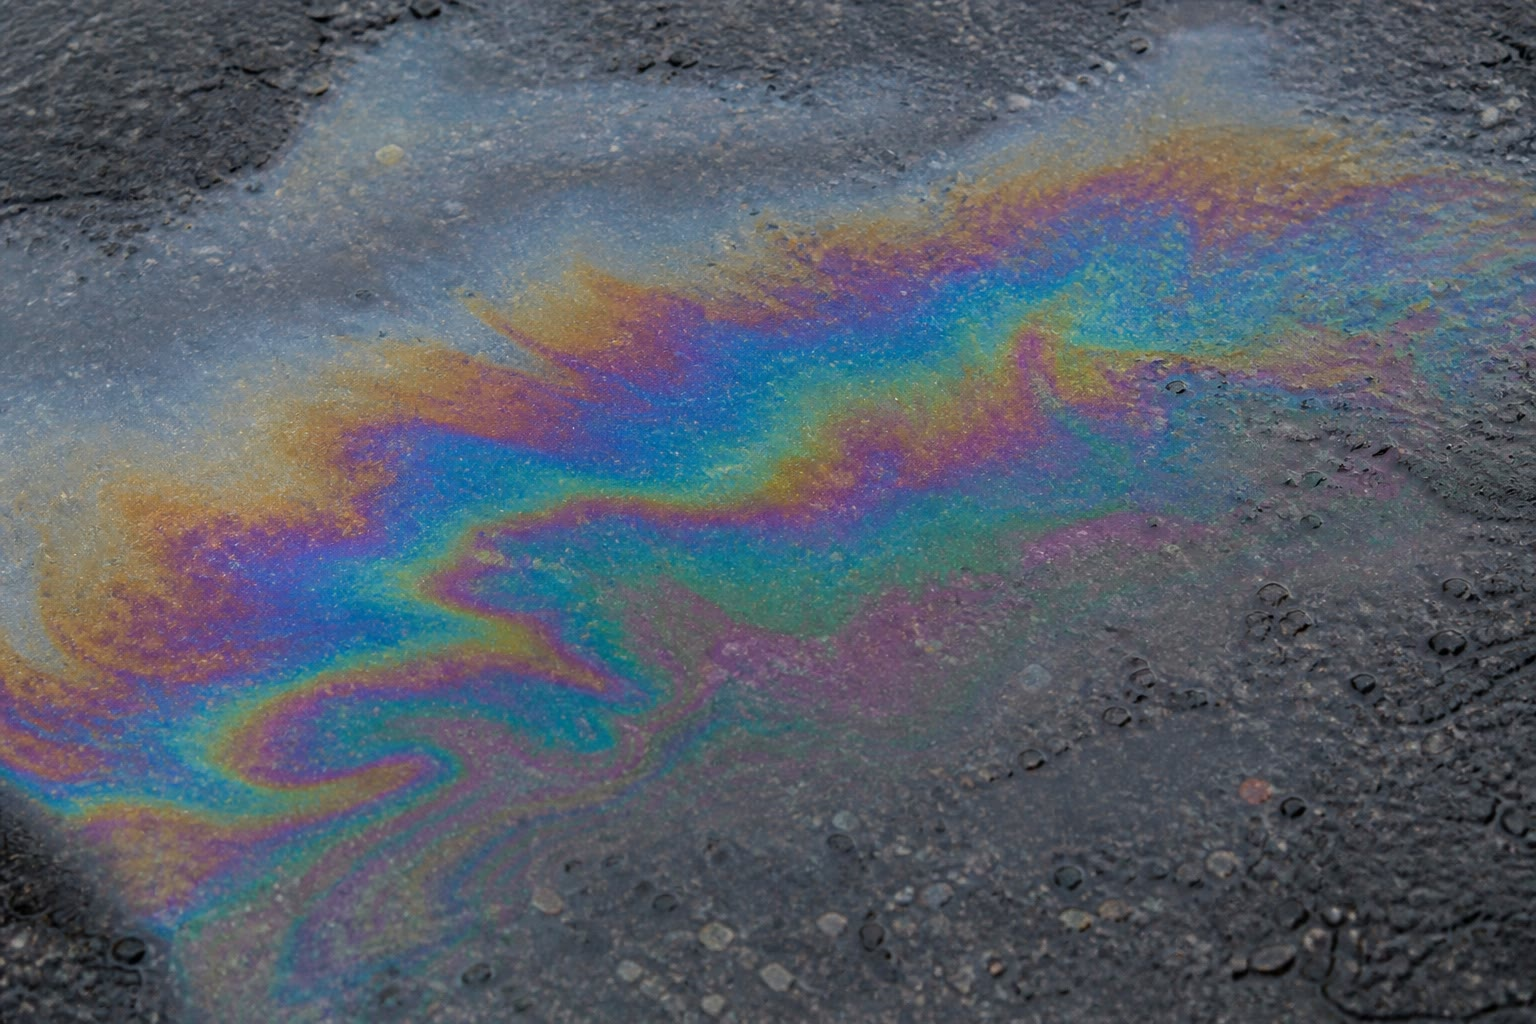
\includegraphics[width=0.58\linewidth]{images/book4/ai/b4-19-oil-film-puddle.jpg}

{\small Un film d'huile sur une route mouillée~: deux réflexions, une par face, et une épaisseur qui varie d'un endroit à l'autre --- chaque couleur brillante là où $2ne$ prend la bonne valeur.}
\end{omfigure}


\section{La formule des interférences}

\begin{theorem}[Interférences à deux ondes]\label{thm:b2:two-wave-interference:formula}
\index{interférences}\index{différence de marche}\index{ordre d'interférence}\index{contraste (franges)}
Deux \omterm{def:b2:scalar-light-model:scalar}{ondes monochromatiques} cohérentes d'intensités $I_1$, $I_2$ et de différence
de phase $\Delta\varphi$ en un point $M$ y donnent l'intensité
\[
I(M) = I_1 + I_2 + 2\sqrt{I_1I_2}\,\cos\Delta\varphi(M) , \qquad
\Delta\varphi = \frac{2\pi}{\lambda_0}\,\delta(M) ,
\]
où $\delta$ est la \emph{\omterm{thm:b2:two-wave-interference:formula}{différence de marche}} optique entre les deux
trajets de la source à $M$. L'intensité est maximale ($I_1 + I_2 +
2\sqrt{I_1I_2}$) là où $\delta = p\lambda_0$, $p$ entier --- l'\emph{\omterm{thm:b2:two-wave-interference:formula}{ordre
d'interférence}} --- et minimale ($I_1 + I_2 - 2\sqrt{I_1I_2}$) là où $\delta = (p +
\tfrac12)\lambda_0$. Le \emph{contraste} (ou visibilité) des franges vaut
\[
V = \frac{I_{\max} - I_{\min}}{I_{\max} + I_{\min}} = \frac{2\sqrt{I_1I_2}}{I_1 + I_2} ,
\]
égal à $1$ pour des intensités égales, cas où les minima sont parfaitement noirs~:
$I = 2I_0(1 + \cos\Delta\varphi) = 4I_0\cos^2(\Delta\varphi/2)$.
\end{theorem}

\begin{proof}
$s = a_1\cos(\omega t - \varphi_1) + a_2\cos(\omega t - \varphi_2)$~; $\langle s^2\rangle$ comme au
\cref{ch:b2:scalar-light-model}, avec $\Delta\varphi$ fixe pendant la
détection~; $I_i = \tfrac12Ka_i^2$. La différence de phase de deux ondes
parties ensemble de la source et ayant parcouru les \omterm{def:b2:scalar-light-model:path}{chemins optiques} $L_1$, $L_2$ vaut
$2\pi(L_2 - L_1)/\lambda_0$ (plus $\pi$ pour chaque réflexion qui inverse le
signe, \cref{ch:b2:wave-interfaces}).
\end{proof}

\begin{remark}[Les trois conditions]\label{rem:b2:two-wave-interference:conditions}
\index{cohérence (spatiale)}\index{cohérence (temporelle)}
Des franges n'existent que si (1) les deux ondes viennent de la \emph{même
source} (deux copies d'une même vibration, sinon $\Delta\varphi$ est aléatoire)~; (2)
la \omterm{thm:b2:two-wave-interference:formula}{différence de marche} est inférieure à la \omterm{prop:b2:scalar-light-model:coherence}{longueur de cohérence}, $|\delta| < \ell_c$
(\emph{cohérence temporelle}~: au-delà les copies appartiennent à des \omterm{prop:b2:scalar-light-model:coherence}{trains
d'ondes} différents)~; (3) la source est assez petite pour que ses différents points
ne produisent pas des systèmes de franges décalés qui se brouillent mutuellement
(\emph{\omterm{prop:b2:two-wave-interference:spatial}{cohérence spatiale}}, ci-dessous). Et une quatrième, généralement satisfaite~: les
deux ondes ne doivent pas avoir des polarisations perpendiculaires (elles s'ajouteraient
en intensité, comme les lampes de poche).
\end{remark}

\section{Les fentes d'Young}

\begin{proposition}[Division du front d'onde~: l'expérience d'Young]\label{prop:b2:two-wave-interference:young}
\index{fentes d'Young}\index{interfrange}\index{division du front d'onde}
Une source ponctuelle $S$ (ou une fente) éclaire deux fentes parallèles étroites
$S_1$, $S_2$ distantes de $a$, équidistantes de $S$~; un écran est placé à
la distance $D \gg a$. Au point de l'écran de hauteur $x$ (parallèlement
à $a$) la \omterm{thm:b2:two-wave-interference:formula}{différence de marche} vaut
\[
\delta = S_2M - S_1M \approx \frac{ax}D ,
\]
et l'écran montre des franges rectilignes équidistantes, brillantes en $x_p =
p\lambda D/a$, avec l'\emph{interfrange}
\[
i = \frac{\lambda D}a .
\]
Les franges existent partout derrière les fentes (elles ne sont \emph{pas
localisées})~; avec une lentille de distance focale $f$ après les fentes, on les
observe dans son plan focal avec $i = \lambda f/a$ (franges «~à l'infini~»).
L'intensité vaut $4I_0\cos^2(\pi ax/\lambda D)$.
\end{proposition}

\begin{proof}
$S_2M^2 - S_1M^2 = [(x + a/2)^2 - (x - a/2)^2] = 2ax$ et $S_2M + S_1M \approx 2D$,
donc $\delta \approx 2ax/2D$. Deux ordres diffèrent de $\lambda$, c'est-à-dire de $\Delta x = \lambda D/a$.
Avec une lentille, les deux ondes qui quittent les fentes sous l'angle $\theta$ avec
l'axe ont la \omterm{thm:b2:two-wave-interference:formula}{différence de marche} $a\sin\theta \approx a\theta$ et se rejoignent en $x = f\theta$.
\end{proof}

\begin{omfigure}
\begin{tikzpicture}[font=\small, x=1cm, y=1cm, >=Stealth]
  \begin{scope}
    \fill (-3.6,0) circle (1.5pt); \node[font=\footnotesize] at (-3.8,0.3) {$S$};
    \draw[thick] (-1.5,-1.6) -- (-1.5,-0.35) (-1.5,-0.15) -- (-1.5,0.15) (-1.5,0.35) -- (-1.5,1.6);
    \fill (-1.5,0.25) circle (1.2pt) node[left, font=\footnotesize] {$S_1$}; \fill (-1.5,-0.25) circle (1.2pt) node[left, font=\footnotesize] {$S_2$};
    \draw[<->] (-1.1,0.25) -- (-1.1,-0.25) node[midway, right, font=\footnotesize] {$a$};
    \draw[thick] (2.8,-1.8) -- (2.8,1.8);
    \fill (2.8,0.9) circle (1.5pt) node[right, font=\footnotesize] {$M$, $x$};
    \draw[omDef, thick] (-1.5,0.25) -- (2.8,0.9); \draw[omDef, thick] (-1.5,-0.25) -- (2.8,0.9);
    \draw[omDef, thick] (-3.6,0) -- (-1.5,0.25); \draw[omDef, thick] (-3.6,0) -- (-1.5,-0.25);
    \draw[<->] (-1.5,-2.0) -- (2.8,-2.0) node[midway, below, font=\footnotesize] {$D$};
    \node[font=\footnotesize] at (0.6,-1.5) {$\delta \approx ax/D$};
    % fringes on the screen
    \foreach \y in {-1.5,-1.0,-0.5,0,0.5,1.0,1.5} \fill[omThm!50] (2.85,{\y-0.12}) rectangle (3.15,{\y+0.12});
    \draw[<->] (3.35,0) -- (3.35,0.5) node[midway, right, font=\footnotesize] {$i$};
  \end{scope}
  \begin{scope}[xshift=9.3cm]
    \begin{axis}[omaxis, axis x line=bottom, axis y line=left, width=4.2cm, height=4.0cm, at={(0,-1.7cm)},
        xlabel={$x/i$}, ylabel={$I/I_0$}, xmin=-2.5, xmax=2.5, ymin=0, ymax=4.4, xtick={-2,-1,0,1,2}, ytick={2,4}, samples=200,
        xlabel style={at={(axis description cs:0.5,-0.14)}, anchor=north},
        ylabel style={at={(axis description cs:-0.12,0.5)}, rotate=90, anchor=south}]
      \addplot[omDef, thick, domain=-2.5:2.5] {4*cos(deg(pi*x))^2};
      \addplot[omThm, thick, dashed, domain=-2.5:2.5] {2+1.2*cos(deg(2*pi*x))};
    \end{axis}
  \end{scope}
\end{tikzpicture}

{\small À gauche~: les \omterm{prop:b2:two-wave-interference:young}{fentes d'Young} --- deux copies de l'onde de la source se rencontrent sur
l'écran avec la \omterm{thm:b2:two-wave-interference:formula}{différence de marche} $ax/D$~; frange brillante tous les
$\lambda D/a$. À droite~: le profil d'intensité, $4I_0\cos^2(\pi x/i)$ pour des ondes
égales (trait plein) et avec un contraste réduit (tirets).}
\end{omfigure}

\begin{example}[Applications numériques, et lumière blanche]\label{ex:b2:two-wave-interference:numbers}
$a = \qty{0.5}{mm}$, $D = \qty{2}{m}$, $\lambda = \qty{600}{nm}$~: $i = \qty{2.4}{mm}$ --- assez
grand pour être vu, ce qui explique que les \omterm{prop:b2:two-wave-interference:young}{fentes d'Young} doivent être proches et l'écran
lointain. En lumière blanche chaque couleur fait ses propres franges, toutes
coïncidant au centre ($\delta = 0$)~: une frange centrale blanche, puis des
franges colorées à mesure que les ordres se séparent (l'interfrange $i$ du rouge vaut $1.8$ fois celui du
violet), et après quelques ordres un champ blanchâtre uniforme --- la
\omterm{prop:b2:scalar-light-model:coherence}{longueur de cohérence} de la lumière blanche est le micromètre, deux ou trois
longueurs d'onde. Un spectromètre braqué sur ce champ «~blanc~» y voit encore
des bandes sombres aux longueurs d'onde pour lesquelles $\delta = (p + \tfrac12)\lambda$~: un
\emph{spectre cannelé}.
\end{example}

\begin{proposition}[Cohérence spatiale~: la source doit être petite]\label{prop:b2:two-wave-interference:spatial}
\index{cohérence spatiale}\index{source étendue}
Chaque point d'une \omterm{prop:b2:two-wave-interference:spatial}{source étendue} produit son propre système de franges~; un
point source décalé transversalement de $b$ à la distance $L$ avant
les fentes décale les franges de $x = bD/L$ (la \omterm{thm:b2:two-wave-interference:formula}{différence de marche} gagne
$ab/L$). Une source de largeur $b$ étale les franges sur un interfrange,
et le contraste s'annule, lorsque
\[
\frac{ab}L \approx \lambda , \qquad\text{c'est-à-dire lorsque les fentes voient la source sous un angle } \frac bL \gtrsim \frac\lambda a .
\]
Les deux fentes doivent se trouver dans l'\emph{aire de cohérence} de la lumière ---
la région sur laquelle l'onde issue de la source a une phase bien définie,
de largeur $\lambda L/b$. La lumière solaire ($b/L = \qty{0.5}{\degree} = \qty{9}{mrad}$)
donne une largeur de cohérence $\lambda/0.009 \approx \qty{60}{\micro m}$~: il fallut à Young un
trou d'épingle pour l'élargir.
\end{proposition}

\begin{proof}
Pour un point source de hauteur $b$, le chemin supplémentaire $SS_2 - SS_1 \approx -ab/L$
s'ajoute à $ax/D$~: le motif se décale de $x = bD/L$. En intégrant les
motifs en $\cos^2$ décalés sur une source de largeur $b$ on obtient un contraste
$|\operatorname{sinc}(\pi ab/\lambda L)|$, nul pour $ab/L = \lambda$.
\end{proof}

\begin{omfigure}
\begin{tikzpicture}[font=\small, x=1cm, y=1cm, >=Stealth]
  \draw[thick, omThm] (-4.2,-0.4) -- (-4.2,0.4); \node[omThm, font=\footnotesize] at (-4.6,0) {$b$};
  \draw[thick] (-1.0,-1.5) -- (-1.0,-0.3) (-1.0,-0.1) -- (-1.0,0.1) (-1.0,0.3) -- (-1.0,1.5);
  \draw[omDef] (-4.2,0.4) -- (-1.0,0.2); \draw[omDef] (-4.2,0.4) -- (-1.0,-0.2);
  \draw[omProp] (-4.2,-0.4) -- (-1.0,0.2); \draw[omProp] (-4.2,-0.4) -- (-1.0,-0.2);
  \draw[<->] (-4.2,-1.9) -- (-1.0,-1.9) node[midway, below, font=\footnotesize] {$L$};
  \draw[thick] (3.0,-1.8) -- (3.0,1.8);
  \foreach \y in {-1.5,-1.0,-0.5,0,0.5,1.0,1.5} \fill[omDef!50] (3.05,{\y-0.1}) rectangle (3.3,{\y+0.1});
  \foreach \y in {-1.5,-1.0,-0.5,0,0.5,1.0,1.5} \fill[omProp!50] (3.35,{\y-0.1+0.25}) rectangle (3.6,{\y+0.1+0.25});
  \node[font=\footnotesize] at (-0.5,2.2) {chaque point source~: ses propres franges, décalées de $bD/L$};
  \node[font=\footnotesize] at (-0.5,-2.5) {contraste perdu quand $ab/L \approx \lambda$};
\end{tikzpicture}

{\small \omterm{prop:b2:two-wave-interference:spatial}{Cohérence spatiale}~: le haut et le bas d'une \omterm{prop:b2:two-wave-interference:spatial}{source étendue}
envoient des systèmes de franges décalés l'un par rapport à l'autre~; quand le décalage
atteint un interfrange le motif est brouillé.}
\end{omfigure}

\section{Lames minces~: division d'amplitude}

\begin{proposition}[Interférences dans une lame mince]\label{prop:b2:two-wave-interference:film}
\index{interférences en lame mince}\index{division d'amplitude}\index{franges d'égale inclinaison}\index{franges d'égale épaisseur}
Une lame d'indice $n$ et d'épaisseur $e$ dans l'air, éclairée sous l'incidence $i$
(angle de réfraction $r$), renvoie deux ondes réfléchies sur ses deux faces,
avec la \omterm{thm:b2:two-wave-interference:formula}{différence de marche}
\[
\delta = 2ne\cos r \ (+\tfrac{\lambda_0}2) ,
\]
la demi-longueur d'onde supplémentaire comptant l'inversion de signe de la réflexion
sur le milieu le plus dense à la première face et non à la seconde
(\cref{ch:b2:wave-interfaces}). Les franges sont brillantes pour $2ne\cos r =
(p + \tfrac12)\lambda_0$, sombres pour $2ne\cos r = p\lambda_0$ --- une lame d'épaisseur
nulle ne réfléchit \emph{rien} (le sommet noir d'un film de savon qui s'écoule).
Pour une lame d'épaisseur uniforme les franges ne dépendent que de $i$
et s'observent à l'infini (anneaux d'\emph{égale inclinaison})~; pour un
coin d'épaisseur lentement variable observé sous incidence quasi normale elles
suivent les lignes de niveau de $e$ et sont localisées sur la lame
(franges d'\emph{égale épaisseur})~: un coin d'air d'angle $\alpha$ montre des
franges rectilignes espacées de $\lambda_0/2\alpha$~; une lentille de rayon $R$ posée sur un plan donne
les \emph{anneaux de Newton}, sombres en $r_p = \sqrt{p\lambda_0R}$.
\end{proposition}

\begin{proof}
Géométrie~: l'onde réfractée à la première face traverse deux fois la lame
($2e/\cos r$ dans le verre, \omterm{def:b2:scalar-light-model:path}{chemin optique} $2ne/\cos r$) tandis que l'onde réfléchie
sur la première face avance de $2e\tan r\sin i$ dans l'air~; la différence vaut
$2ne/\cos r - 2e\tan r\sin i = 2ne\cos r$ avec $\sin i = n\sin r$. Pour le
coin, $e = \alpha x$ et les franges sombres successives en $2\alpha x = p\lambda$~; pour la
lentille, $e \approx r^2/2R$.
\end{proof}

\begin{omfigure}
\begin{tikzpicture}[font=\small, x=1cm, y=1cm, >=Stealth]
  \begin{scope}
    \fill[omDef!15] (-3,-0.9) rectangle (3,0.9); \draw[thick] (-3,0.9) -- (3,0.9) (-3,-0.9) -- (3,-0.9);
    \node[font=\footnotesize] at (2.4,0) {$n$}; \draw[<->] (-2.7,-0.9) -- (-2.7,0.9) node[midway, left, font=\footnotesize] {$e$};
    \draw[omThm, thick, ->] (-2.2,2.2) -- (-0.9,0.95);
    \draw[omThm, thick, ->] (-0.85,0.92) -- (0.4,2.2);
    \draw[omProp, thick] (-0.9,0.9) -- (-0.2,-0.9) -- (0.5,0.9);
    \draw[omProp, thick, ->] (0.5,0.92) -- (1.75,2.2);
    \node[font=\footnotesize] at (-1.7,1.85) {$i$}; \node[font=\footnotesize] at (-0.75,-0.0) {$r$};
    \node[font=\footnotesize] at (0,-1.4) {$\delta = 2ne\cos r$ (+ $\lambda/2$)};
  \end{scope}
  \begin{scope}[xshift=7.8cm]
    \draw[thick] (-2.6,0) -- (2.6,0);
    \draw[thick] (-2.6,0.05) arc[start angle=-90, end angle=-60, radius=14] ;
    \draw[thick] (-2.6,0.05) -- (2.6,0.55);
    \foreach \x in {-2.0,-1.3,-0.6,0.1,0.8,1.5,2.2} \draw[omThm, very thick] (\x,-0.25) -- (\x,-0.45);
    \node[font=\footnotesize] at (0,-0.85) {coin d'air~: frange sombre tous les $\lambda/2\alpha$};
    \draw[omDef, thick] (-2.6,0.05) -- (-2.6,0); \node[font=\footnotesize] at (2.9,0.3) {$\alpha$};
  \end{scope}
\end{tikzpicture}

{\small À gauche~: les deux réflexions sur une lame mince --- une par
face, la seconde retardée par la double traversée. À droite~: un coin d'air
entre deux lames montre des franges rectilignes d'égale épaisseur, une par
demi-longueur d'onde d'épaisseur supplémentaire.}
\end{omfigure}

\begin{example}[Savon, huile, libellules]\label{ex:b2:two-wave-interference:colours}
Un film de savon ($n = 1.33$) de \qty{300}{nm} d'épaisseur vu sous incidence normale~:
brillant pour $2ne = (p + \tfrac12)\lambda$, c'est-à-dire $\lambda = 798/(p + \tfrac12)$ nm~: \qty{532}{nm}
(vert, $p = 1$) dans le visible, et une bande sombre à \qty{400}{nm}~; le
film paraît vert. À mesure qu'il s'écoule et s'amincit, la couleur parcourt la
séquence et finit noire. Un film d'huile (\qty{400}{nm}, $n = 1.45$) sur l'eau
($1.33$)~: la seconde réflexion, vers un indice plus bas, n'inverse pas
le signe, de sorte qu'ici encore $\delta = 2ne + \lambda/2$ et que le film est brillant pour $2ne =
(p + \tfrac12)\lambda$~: \qty{464}{nm} ($p = 2$), du bleu. L'irisation d'une aile
de papillon, d'une carapace de scarabée ou d'un disque compact sont des interférences
de même nature (celle du disque, à ondes multiples~: \cref{ch:b2:gratings}),
ce qui explique qu'elles changent avec l'angle --- $\delta$ dépend de $\cos r$ ---
alors que la couleur d'un pigment, non.
\end{example}

\begin{method}[Résoudre un problème d'interférences]\label{met:b2:two-wave-interference:method}
(1) Repérer les deux trajets de la source à $M$ et calculer la
\omterm{thm:b2:two-wave-interference:formula}{différence de marche} optique $\delta(M)$, en ajoutant $\lambda/2$ pour chaque réflexion
avec inversion de signe. (2) $I = I_1 + I_2 + 2\sqrt{I_1I_2}\cos(2\pi\delta/\lambda)$~;
brillant en $\delta = p\lambda$. (3) L'interfrange par $\delta(M + \Delta M) - \delta(M) =
\lambda$. (4) Vérifier la cohérence temporelle ($\delta_{\max} < \ell_c$, nombre de
franges visibles $\sim\lambda/\Delta\lambda$) et la \omterm{prop:b2:two-wave-interference:spatial}{cohérence spatiale} (angle de la source
$< \lambda/a$). (5) Dire où les franges sont localisées (partout pour deux
sources ponctuelles~; sur la lame pour les \omterm{prop:b2:two-wave-interference:film}{franges d'égale épaisseur}~; à l'infini
pour celles d'égale inclinaison).
\end{method}

\section{Exercices}

\begin{exercise}[$\star$]\label{exo:b2:two-wave-interference:1}
\omterm{prop:b2:two-wave-interference:young}{Fentes d'Young} distantes de $a = \qty{0.40}{mm}$, écran à $D = \qty{1.5}{m}$, $\lambda =
\qty{633}{nm}$~: interfrange~; ordre de la frange en $x = \qty{1.0}{cm}$~; position
de la dixième frange sombre~; interfrange avec des fentes distantes de \qty{2}{mm},
et dans l'eau ($n = 1.33$).
\end{exercise}

\begin{exercise}[$\star$]\label{exo:b2:two-wave-interference:2}
Deux ondes d'intensités $I_0$ et $I_0/4$ interfèrent~: $I_{\max}$, $I_{\min}$,
contraste. Idem pour $I_0$ et $I_0/100$~: pourquoi les franges restent-elles visibles
avec des faisceaux aussi inégaux~? Une des deux \omterm{prop:b2:two-wave-interference:young}{fentes d'Young} est recouverte d'un
filtre gris transmettant $50\%$~: nouveau contraste.
\end{exercise}

\begin{exercise}[$\star$]\label{exo:b2:two-wave-interference:3}
Un film de savon de \qty{250}{nm} d'épaisseur ($n = 1.33$) vu sous incidence normale~:
longueurs d'onde visibles les plus et les moins réfléchies~; sa couleur. Un film de
\qty{1.0}{\micro m}~: combien de longueurs d'onde brillantes dans le visible, et que
voit l'œil~?
\end{exercise}

\begin{exercise}[$\star$]\label{exo:b2:two-wave-interference:4}
Anneaux de Newton entre une lentille de rayon $R = \qty{2.0}{m}$ et un plan, en
lumière de sodium~: rayons des trois premiers anneaux sombres~; nombre d'anneaux
dans un rayon de \qty{1}{cm}~; le centre est-il brillant ou sombre, et pourquoi~?
Qu'est-ce qui change si l'on remplit l'intervalle d'eau~?
\end{exercise}

\begin{exercise}[$\star\star$]\label{exo:b2:two-wave-interference:5}
\emph{Lumière blanche.} \omterm{prop:b2:two-wave-interference:young}{Fentes d'Young} en lumière blanche ($400$ à \qty{700}{nm}),
$a = \qty{0.5}{mm}$, $D = \qty{1}{m}$. (a) Interfrange pour le violet et pour le rouge~;
position des deuxième frange brillante rouge et troisième violette. (b)
Au-delà de quel ordre les franges rouge et violette d'ordres successifs se recouvrent-elles~? (c)
En $x = \qty{5}{mm}$, quelles longueurs d'onde manquent
(spectre cannelé)~? (d) Expliquer la suite des couleurs vues du
centre vers l'extérieur.
\end{exercise}

\begin{exercise}[$\star\star$]\label{exo:b2:two-wave-interference:6}
\emph{Taille de la source.} Une lampe au sodium éclaire des \omterm{prop:b2:two-wave-interference:young}{fentes d'Young} ($a = \qty{1.0}{mm}$)
à travers une fente source placée à $L = \qty{40}{cm}$. (a) Largeur maximale de la
fente source pour un bon contraste (prendre $ab/L < \lambda/4$). (b) La fente source
est élargie à \qty{0.5}{mm}~: contraste (utiliser $|\operatorname{sinc}(\pi ab/\lambda L)|$).
(c) Pourquoi ne peut-on pas simplement utiliser la lampe nue (largeur \qty{1}{cm})~? (d) Le
Soleil comme source, de \qty{9}{mrad} de diamètre apparent~: écartement maximal des fentes qui
donne des franges.
\end{exercise}

\begin{exercise}[$\star\star$]\label{exo:b2:two-wave-interference:7}
\emph{Miroir de Lloyd.} Une source ponctuelle à la hauteur $h = \qty{0.2}{mm}$ au-dessus d'un
miroir plan, écran à $D = \qty{1.0}{m}$, $\lambda = \qty{500}{nm}$~: l'onde directe
interfère avec celle que réfléchit le miroir (une source virtuelle en
$-h$). (a) Interfrange. (b) La frange située au bord du miroir ($x = 0$) est
sombre~: qu'est-ce que cela apprend sur la réflexion~? (c) Nombre de franges
visibles si la \omterm{prop:b2:scalar-light-model:coherence}{longueur de cohérence} de la source vaut \qty{50}{\micro m}. (d) Pourquoi ce
montage est-il l'«~interféromètre marin~» du radioastronome pour une étoile qui se lève~?
\end{exercise}

\begin{exercise}[$\star\star$]\label{exo:b2:two-wave-interference:8}
\emph{Coin d'air.} Deux lames de verre de \qty{10}{cm} de long se touchent à une extrémité et
sont écartées à l'autre par un cheveu de diamètre $d$~; en lumière de sodium
on compte $42$ franges sombres. (a) $d$. (b) Interfrange. (c) L'intervalle
est rempli d'eau~: nombre de franges. (d) On presse légèrement les lames à l'extrémité écartée~: que font
les franges, et quelle précision sur
$d$ donne le comptage d'un quart de frange~?
\end{exercise}

\begin{exercise}[$\star\star$]\label{exo:b2:two-wave-interference:9}
\emph{Huile sur eau.} Un film d'huile ($n = 1.45$) d'épaisseur $e$ flotte
sur de l'eau ($n = 1.33$). (a) Laquelle des deux réflexions inverse le
signe~? \omterm{thm:b2:two-wave-interference:formula}{Différence de marche}. (b) Pour $e = \qty{400}{nm}$ sous incidence normale~:
longueurs d'onde réfléchies renforcées et annulées~; couleur. (c) Film le plus mince
qui paraisse violet (\qty{420}{nm}). (d) Pourquoi les couleurs se déplacent-elles vers
le bleu quand on regarde le film obliquement~? (e) Qu'est-ce qui change pour un film
dont l'indice se situe \emph{entre} ceux des deux milieux (un traitement sur du
verre)~?
\end{exercise}

\begin{exercise}[$\star\star\star$]\label{exo:b2:two-wave-interference:10}
\emph{Une lame sur une fente.} Une lame de verre d'épaisseur $e = \qty{20}{\micro m}$
et d'indice $1.5$ recouvre la fente $S_1$ d'une paire d'Young ($a = \qty{1}{mm}$, $D =
\qty{2}{m}$, $\lambda = \qty{500}{nm}$). (a) \omterm{def:b2:scalar-light-model:path}{Chemin optique} supplémentaire~; de combien de franges
et dans quel sens le motif se décale-t-il~? (b) En lumière blanche,
où va la frange centrale blanche (désormais déplacée) --- est-elle encore
visible~? \omterm{prop:b2:scalar-light-model:coherence}{Longueur de cohérence} \qty{1.5}{\micro m}. (c) Utiliser le motif en lumière
blanche pour mesurer $e$~: comment~? (d) On incline la lame~: le décalage croît
--- montrer qu'au premier ordre il croît comme $e(n - 1)\theta^2/2 \times (1 + 1/n)$
et l'estimer pour \qty{5}{\degree}.
\end{exercise}

\begin{exercise}[$\star\star\star$]\label{exo:b2:two-wave-interference:11}
\emph{L'interféromètre stellaire.} Deux miroirs distants de $a$
recueillent la lumière d'une étoile et la font interférer. L'étoile est un
disque uniforme de diamètre angulaire $\theta$~; chaque point du disque décale les
franges, et le contraste s'annule pour $a = 1.22\lambda/\theta$ (admis, version pour un
disque de $ab/L = \lambda$). (a) Bételgeuse, $\theta = \qty{0.047}{''}$
(secondes d'arc), $\lambda = \qty{570}{nm}$~: base pour laquelle les franges
disparaissent (Michelson, 1920, au mont Wilson). (b) Pourquoi un unique
télescope de \qty{2.5}{m} ne résout-il pas le disque (sa limite vaut $1.22\lambda/d$)~?
(c) Les interféromètres modernes relient des télescopes distants de \qty{100}{m}~: plus petit
diamètre mesurable. (d) Pourquoi les deux trajets doivent-ils être égaux à mieux que la
\omterm{prop:b2:scalar-light-model:coherence}{longueur de cohérence}, et combien vaut celle-ci pour un filtre de \qty{10}{nm}~?
\end{exercise}

\begin{exercise}[$\star\star\star$]\label{exo:b2:two-wave-interference:12}
\emph{Anneaux d'égale inclinaison.} Une lame à faces parallèles d'épaisseur $e =
\qty{2.0}{mm}$ et d'indice $1.5$ est éclairée par une large source au sodium~; la
lumière réfléchie est focalisée par une lentille de $f = \qty{50}{cm}$. (a) Montrer que les
anneaux se trouvent aux angles $i_p$ vérifiant $2ne\cos r_p = (p + \tfrac12)\lambda$ (brillants)
et qu'au voisinage du centre $\cos r \approx 1 - i^2/2n^2$. (b) Ordre au
centre~; le centre est-il brillant~? (c) Rayons des trois premiers anneaux
brillants dans le plan focal. (d) Pourquoi ces anneaux s'observent-ils avec une
\omterm{prop:b2:two-wave-interference:spatial}{source étendue} alors que les franges d'Young exigent une source étroite~? (Localisation
à l'infini.)
\end{exercise}

\begin{omfigure}
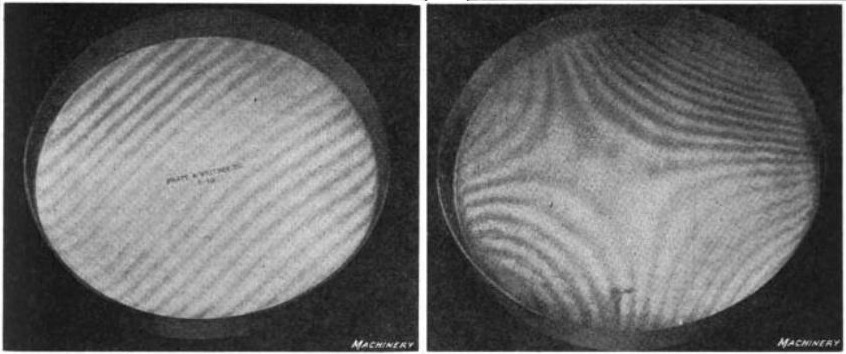
\includegraphics[width=0.62\linewidth]{images/book4/optical-flat-fringes.jpg}

{\small \omterm{prop:b2:two-wave-interference:film}{Franges d'égale épaisseur} entre un plan optique et une surface d'acier à contrôler, sur une photographie d'ajusteur des années 1915~: franges rectilignes sur une surface plane, incurvées là où elle est usée --- chaque frange une marche d'une demi-longueur d'onde.}
\end{omfigure}

\section{Problème~: les miroirs de Fresnel et un film d'huile}

\begin{problem}[{Problème du week-end --- un interféromètre de 1816 et un
arc-en-ciel sur une flaque~: deux façons de diviser une onde et les deux
cohérences qui limitent les deux}]
\label{pb:b2:two-wave-interference:1}

\medskip
\noindent\textbf{Partie I --- Les miroirs de Fresnel.}
Deux miroirs plans se touchant selon une arête font un très petit angle $\alpha =
\qty{5.0e-3}{rad}$~; une fente source $S$, parallèle à cette arête, est à $d =
\qty{20}{cm}$ de celle-ci, et l'écran à $D = \qty{1.5}{m}$ au-delà. $\lambda =
\qty{589}{nm}$ (sodium).
\begin{enumerate}
  \item Montrer que les deux miroirs donnent deux images virtuelles $S_1$, $S_2$ de
        $S$ sur un cercle de rayon $d$ centré sur l'arête de contact,
        distantes de $a = 2\alpha d$~; valeur.
  \item Pourquoi les ondes issues de $S_1$ et $S_2$ interfèrent-elles, alors que celles de
        deux lampes distinctes ne le feraient pas~?
  \item Interfrange sur l'écran (distance des sources à
        l'écran $\approx d + D$)~; nombre de franges sur la
        zone large de \qty{5}{mm} où les deux faisceaux réfléchis se recouvrent.
  \item \omterm{thm:b2:two-wave-interference:formula}{Ordre d'interférence} au bord de cette zone~; est-il en deçà
        de la limite fixée par la \omterm{prop:b2:scalar-light-model:coherence}{longueur de cohérence} de la lampe (\qty{2}{cm})~?
  \item La fente source fait \qty{20}{\micro m} de large~: décalage des franges
        produites par ses deux bords (chaque point source est imagé en deux
        points virtuels~; le système de franges se décale de $bD'/d$ avec $D' =
        d + D$)~; le contraste est-il conservé (comparer à $i$)~?
  \item La fente est élargie à \qty{0.1}{mm}~: contraste, à l'aide de
        $|\operatorname{sinc}(\pi ab/\lambda d)|$.
  \item Les deux miroirs réfléchissent $90\%$ et $80\%$ de la lumière~: contraste
        des franges.
  \item Une lame de verre de \qty{10}{\micro m} d'épaisseur ($n = 1.5$) est placée
        devant un des miroirs~: décalage du motif, en franges~; peut-on le
        suivre en lumière de sodium~? En lumière blanche~?
  \item On remplace la lampe au sodium par de la lumière blanche~: décrire l'écran~;
        combien de franges colorées de chaque côté du centre~?
\end{enumerate}

\medskip
\noindent\textbf{Partie II --- Le film d'huile.}
Un film d'huile ($n = 1.45$) s'étale sur une route mouillée ($n_{\text{eau}} = 1.33$),
éclairé par un ciel couvert et observé sous incidence quasi normale.
\begin{enumerate}[resume]
  \item Réflexions sur les deux faces~: laquelle inverse le signe~? \omterm{thm:b2:two-wave-interference:formula}{Différence
        de marche}~; condition pour une couleur brillante.
  \item Épaisseur de la région la plus mince qui paraisse rouge ($\lambda =
        \qty{650}{nm}$)~; verte (\qty{550}{nm})~; violette (\qty{420}{nm}).
  \item Une région de \qty{600}{nm} d'épaisseur~: quelles longueurs d'onde visibles sont
        renforcées, lesquelles annulées~; sa couleur.
  \item Pourquoi le film montre-t-il des bandes colorées (qu'est-ce qui varie le long de la
        route), et pourquoi les bandes suivent-elles les lignes de niveau d'épaisseur~?
  \item Le film s'amincit par évaporation~: décrire l'évolution de la
        couleur en un point donné~; que voit-on quand $e \to 0$
        ici --- brillant ou sombre~? Comparer avec un film de savon dans l'air.
  \item Le sommet d'un film de savon qui s'écoule devient noir juste avant
        d'éclater~: épaisseur en ce point (quelques nanomètres) et pourquoi noir.
  \item Vu sous \qty{60}{\degree} d'incidence~: angle de réfraction dans l'huile,
        et décalage des longueurs d'onde brillantes de la question 11.
  \item Au-delà de quelle épaisseur les couleurs s'estompent-elles en un gris
        uniforme, pour une lumière du jour de \omterm{prop:b2:scalar-light-model:coherence}{longueur de cohérence} voisine de \qty{1}{\micro m}~?
  \item La lumière du ciel n'est pas polarisée et arrive de nombreuses
        directions~: pourquoi le motif ne se brouille-t-il pas comme une \omterm{prop:b2:two-wave-interference:spatial}{source étendue}
        brouille les franges d'Young~? (Localisation sur la lame.)
\end{enumerate}

\medskip
\noindent\textbf{Partie III --- Les deux cohérences.}
\begin{enumerate}[resume]
  \item Cohérence temporelle~: pour les miroirs de Fresnel en lumière de sodium,
        l'ordre maximal visible~; avec un laser ($\ell_c = \qty{10}{m}$).
  \item \omterm{prop:b2:two-wave-interference:spatial}{Cohérence spatiale}~: la largeur maximale de source pour les miroirs
        (d'après $ab/d < \lambda/4$) et pour les \omterm{prop:b2:two-wave-interference:young}{fentes d'Young} avec $a = \qty{1}{mm}$ à
        $L = \qty{40}{cm}$.
  \item Expliquer pourquoi la lame mince tolère une \omterm{prop:b2:two-wave-interference:spatial}{source étendue} alors que
        les \omterm{prop:b2:two-wave-interference:young}{fentes d'Young} ne le font pas~: tracer les deux rayons de la lame pour deux
        points sources différents et montrer qu'ils se rejoignent encore sur la lame.
  \item La raie du sodium fait elle-même \qty{0.02}{nm} de large~: combien de franges
        les miroirs peuvent-ils montrer au plus (utiliser $N \approx \lambda/\Delta\lambda$)~?
  \item Un étudiant remplace la lampe au sodium par une DEL verte ($\Delta\lambda =
        \qty{30}{nm}$)~: nombre de franges visibles avec les miroirs.
  \item Avec un laser les franges couvrent toute la zone de recouvrement
        avec un contraste maximal, mais l'écran est «~granuleux~»~: pourquoi~?
  \item En un tableau, pour les miroirs et la lame~: comment l'onde est
        divisée, où les franges sont localisées, ce qui limite leur
        nombre, et ce que fait une source plus large.
\end{enumerate}
\end{problem}
